%%%%%%%%%%%%%%%%%%%%%%%%%%%%%%%%%%%%%%%%%%%%%%%%%%%%%%%%%%%%%%%%%%%%%%%%
% RevTeX 4.1 LaTeX
% Kevin C. Young
% Scalable & Secure Systems Research (08961)
% Thu Mar  5 15:29:19 PST 2015
%%%%%%%%%%%%%%%%%%%%%%%%%%%%%%%%%%%%%%%%%%%%%%%%%%%%%%%%%%%%%%%%%%%%%%%%

\documentclass[aps,nofootinbib,pra,notitlepage,twocolumn]{revtex4-1}
\usepackage{amsfonts,amsmath,amssymb,amsthm}
 \usepackage{array,bm,color}
\usepackage{epsfig,graphicx,nomencl,revsymb4-1,upgreek,url}
\usepackage{hyperref}
\usepackage{algorithm}
\usepackage{algpseudocode}
\usepackage{graphicx}
\usepackage{calc}
\graphicspath{{./figures/}}
\hypersetup{colorlinks=true, pdfauthor=Kevin C. Young, pdftitle=Decorrelating Errors}
\newcommand{\tr}{{\rm Tr\thinspace}}
\newcommand{\bra}[1]{\ensuremath{\left\langle{#1}\right\vert}}
\newcommand{\ket}[1]{\ensuremath{\left\vert{#1}\right\rangle}}
\newcommand{\braket}[2]{\left\langle #1 | #2 \right\rangle}
\newcommand{\ketbra}[2]{\left| #1 \right\rangle\!\!\!\,\left\langle #2 \right|}
\newcommand{\abs}[1]{\left\vert #1 \right\vert}
\newcommand{\expect}[1]{\ensuremath{\left\langle{#1}\right\rangle}}
\newcommand{\timeorder}{\ensuremath{\underset{\leftarrow}{\mathcal{T}}}}
\newcommand{\ident}{{\mathbb1}}
\newcommand{\order}[1]{\mathcal{O}\left( #1 \right)}
\newcommand{\diag}[1]{\mathrm{diag}\{#1\}}
\newcommand{\trans}[1]{#1^\mathsf{T}}
\newcommand{\T}{\mathsf{T}}
\newcommand{\erf}[1]{Eq.~(\ref{#1})}
\newcommand{\needcite}{{\color{blue}\textsuperscript{[citation needed]}}}
\newcommand{\note}[1]{{\color{red}[#1]}}
\newcommand{\kcy}[1]{{\color{red}[#1]_{\rm{KCY}}}}
\newcommand{\amp}[1]{{\color{red}[#1]_{\rm{AMP}}}}

\newcommand{\actual}{\ensuremath{\tilde{\mathcal{G}}}}
\newcommand{\target}{\ensuremath{{\mathcal{G}}}}
\newcommand{\error}{\ensuremath{{\mathcal{E}}}}

%-------------Header begins here----------------------------------------
\begin{document}
\title{Advantages of mixed unitary operators for quantum information processing}

\author{Anthony M. Polloreno}
\email[Email: ]{anthony@rigetti.com}
\affiliation{Rigetti Computing, Berkeley, CA}

\author{Kevin C. Young}
\affiliation{Sandia National Laboratories, Livermore, CA}

\date{\today}

\begin{abstract}
Coherent errors in quantum operations are ubiquitous. Whether arising from spurious environmental couplings or errors in control fields, such errors can accumulate rapidly and degrade the performance of a quantum circuit significantly more than an average gate fidelity may indicate. As Hastings and Campbell have recently shown, randomly sampling an ensemble of implementations of a target gate yields an effective quantum channel that well-approximates the target, but with dramatically suppressed coherent error. Our results extend those of Hastings and Campbell to include robustness to drifting external control parameters. We implement these constructions using a superconducting qubit and will discuss randomized benchmarking results consistent with a marked reduction in coherent error.
\end{abstract}

\pacs{}

\maketitle


% ==============================================================================
% Section: Introduction
% ==============================================================================
\section{Introduction}
\label{sec:introduction}

The past decade has seen a dramatic increase in the performance and scale of quantum information processors (QIPs). Gate fidelities are now routinely in the 99\% to 99.99\% range \cite{Barends2014, Ballance2016}, and dozens of individually-addressable qubits are becoming available on integrated devices. While these advances represent important steps forward on the path towards a computationally useful QIP, the quantum advantage milestone \cite{1203.5813} has yet to be definitively reached. The limiting factor, of course, is errors in the quantum gate operations.

The impact of an error in a quantum gate depends strongly on both the magnitude and the nature of the errors. Systematic, or \emph{coherent}, errors can arise from poorly calibrated controls or imperfect gate compilations that induce repeatable, undesired unitary errors on the state of a QIP. Errors of this type are correlated in time and add up coherently. They are are  computationally expensive to model and it is difficult to place tight analytic bounds on circuit performance. Contrast this against random, or \emph{stochastic}, errors, which result from high-frequency noise in the controls or the environment. Systems with stochastic errors can be  modeled by defining a rate of various discrete errors in the system, such as a bit flip or phase flip. These errors are significantly easier to simulate on a classical computer, and their impact on quantum circuits is much easier to estimate.

Despite the relative ease of modeling stochastic errors, coherent errors are often much more likely to appear in QIPs. While these errors can often be reconstructed using various tomographic techniques, their impact is difficult to predict. The diamond distance can be used to bound the total variation distance (TVD) of a quantum circuit, but it is in general sensitive at first order to repeated application of gate with coherent errors. For long circuits, this can add up extremely quickly. Recent work by Campbell and Hastings\cite{Campbell2017, 1612.01011, 1811.08017}, however, has shown that coherent noise can be strongly suppressed by probabilistically mixing several distinct implementations of the target quantum gates. The resulting effective quantum process has a diamond distance that grows only quadratically in the over/under rotation angle of the component gates.

%Drifting control parameters or environmental variables can easily have long correlation times that result in errors which are strongly coherent over the length of a quantum circuit. 

In this article we discuss various applications of these mixed unitary controls, and show that the advantages of this approach can be made robust to drift in the target gates. We demonstrate that, depending on the objective, different numerical optimzations may be prefered. We present an experimental implementation of single-qubit mixed unitary controls on a superconducting qubit testbed at Rigetti Computing. Using randomized benchmarking, we are able to show a marked improvement in error rates, as well as a reduced variance in circuit outcome probabilities, indicating a reduction in the coherence of the error. We further provide an optimal control approach to the mixed unitary control design problem, and apply our methods in simulation where we construct single- and two-qubit mixed unitary controls which are robust to drift and uncertainty in the control parameters.   

% For instance, the repeated measurements that occur in quantum error correction are suspected to reduce the potential impact of coherent buildup of error. Modern devices, however, do not have sufficient numbers of qubits and their errors are above the threshold at which QEC becomes a viable option.


% ==============================================================================
% Section: Mathematical preliminaries
% ==============================================================================
\section{Mathematical preliminaries}
\label{sec:representing_quantum_gates}
Quantum gate operations are implemented by applying a sequence of classical control fields to some set of qubits. Fluctuations in the environment or imperfections in the controls can cause the state of the qubits to change in a way that is different from what was intended.  But if the gates are fairly stable with time and context\cite{1810.05651}, then we can usually describe their action on the qubit state using \emph{process matrices} -- linear, Markovian maps on the state of some qubits.  When working with process matrices, it is convenient to write the system density operator using a vectorized representation, and in this article, we'll make use of the generalized Bloch vector,
\begin{equation}
  \vec \rho = \tr(\rho \vec \Sigma),
\end{equation}
where $\vec \Sigma$ is a vector of all $4^n$ $n$-qubit Pauli operators. The action of a gate is then given by the usual matrix multiplication:
\begin{equation}\label{error_def}
  \vec\rho \rightarrow \target\vec\rho = \error \actual \vec\rho.
\end{equation}
Here $\target$ is the target operation, $\actual$ is the actual gate as implemented, and $\error$ is the effective error channel:

\begin{equation}\label{eq:process_matrix}
\error =
	\left(\begin{array}{c|cccc}
		1 &  & \vec{0}^T & \\ 
		\hline & &  &  \\
		\vec{m} &  & R &  \\
		 &  &  & 
	\end{array} 	
	\right)
\end{equation}
The top row of all trace-preserving (TP) maps is fixed to $\{1,0,0,0,\cdots\}$.  The rest of the first column, $\vec{m}$, describes any deviations from unitality, as could arise from amplitude damping. If the error channel is unitary, then the error is coherent, and the submatrix $R$ is perfectly antisymmetric, corresponding to a rotation of the generalized Bloch vector. If  $R$ is diagonal, then the error channel is Pauli stochastic, with each entry  corresponding to the probability that the associated Pauli error occurs in each application of the gate. That is to say that $\error_{ii}$ gives the probability that the following map is applied:
\begin{equation}
\vec\rho \rightarrow \tr{(\sigma_j^{\dagger}\sigma_i\sigma_k\sigma_i^{\dagger})}\vec{\rho}
\end{equation}
 If R is symmetric but not diagonal, then the channel is still stochastic, but the random errors consist of correlated Pauli operators (such as $X+Y$). For a single qubit, this describes everything, but the situation can be slightly more complicated for more qubits. 

For a collection of single qubit controls $\{U_i\}$ generated by $\{H_i\}$, the channel that results in general has elements:
\begin{align}
	\mathcal{M}_{jk} 
		=& \sum_i p_i \tr{(\sigma_j^{\dagger}U\sigma_kU^{\dagger})} \\
		=& \sum_i p_i \tr{(\sigma_j^{\dagger} \exp(i \frac{\theta_i}{2} H_i)\sigma_k		\exp(-i \frac{\theta_i}{2} H_i)}) \\
		=& \tr{\sum_i p_i (\sigma_j^{\dagger} (\cos\theta_i + i \sin\theta_i H_i) \sigma_k		(\cos\theta_i - i \sin\theta_i H_i))} \\
		=& \tr (\sum_i p_i (\sigma_j\sigma_k\cos\theta_i^2 + \sigma_jH_i\sigma_k H_i\sin\theta_i^2 \\ 
		&+ iH_i\sigma_k\sin\theta_i\cos\theta_i - i\sigma_j H_i\sin\theta_i\cos\theta_i))
\end{align}
The first term corresponds to the identity, and $\sin\theta^2$ is always positive, so we cannot hope to eliminate the second term, but $\sin\theta\cos\theta$ may be positive or negative, and so there is hope that we could possibly combine various implementations to eliminate this term. The result would be a purely stochastic channel. 

\begin{figure}
  \centering
  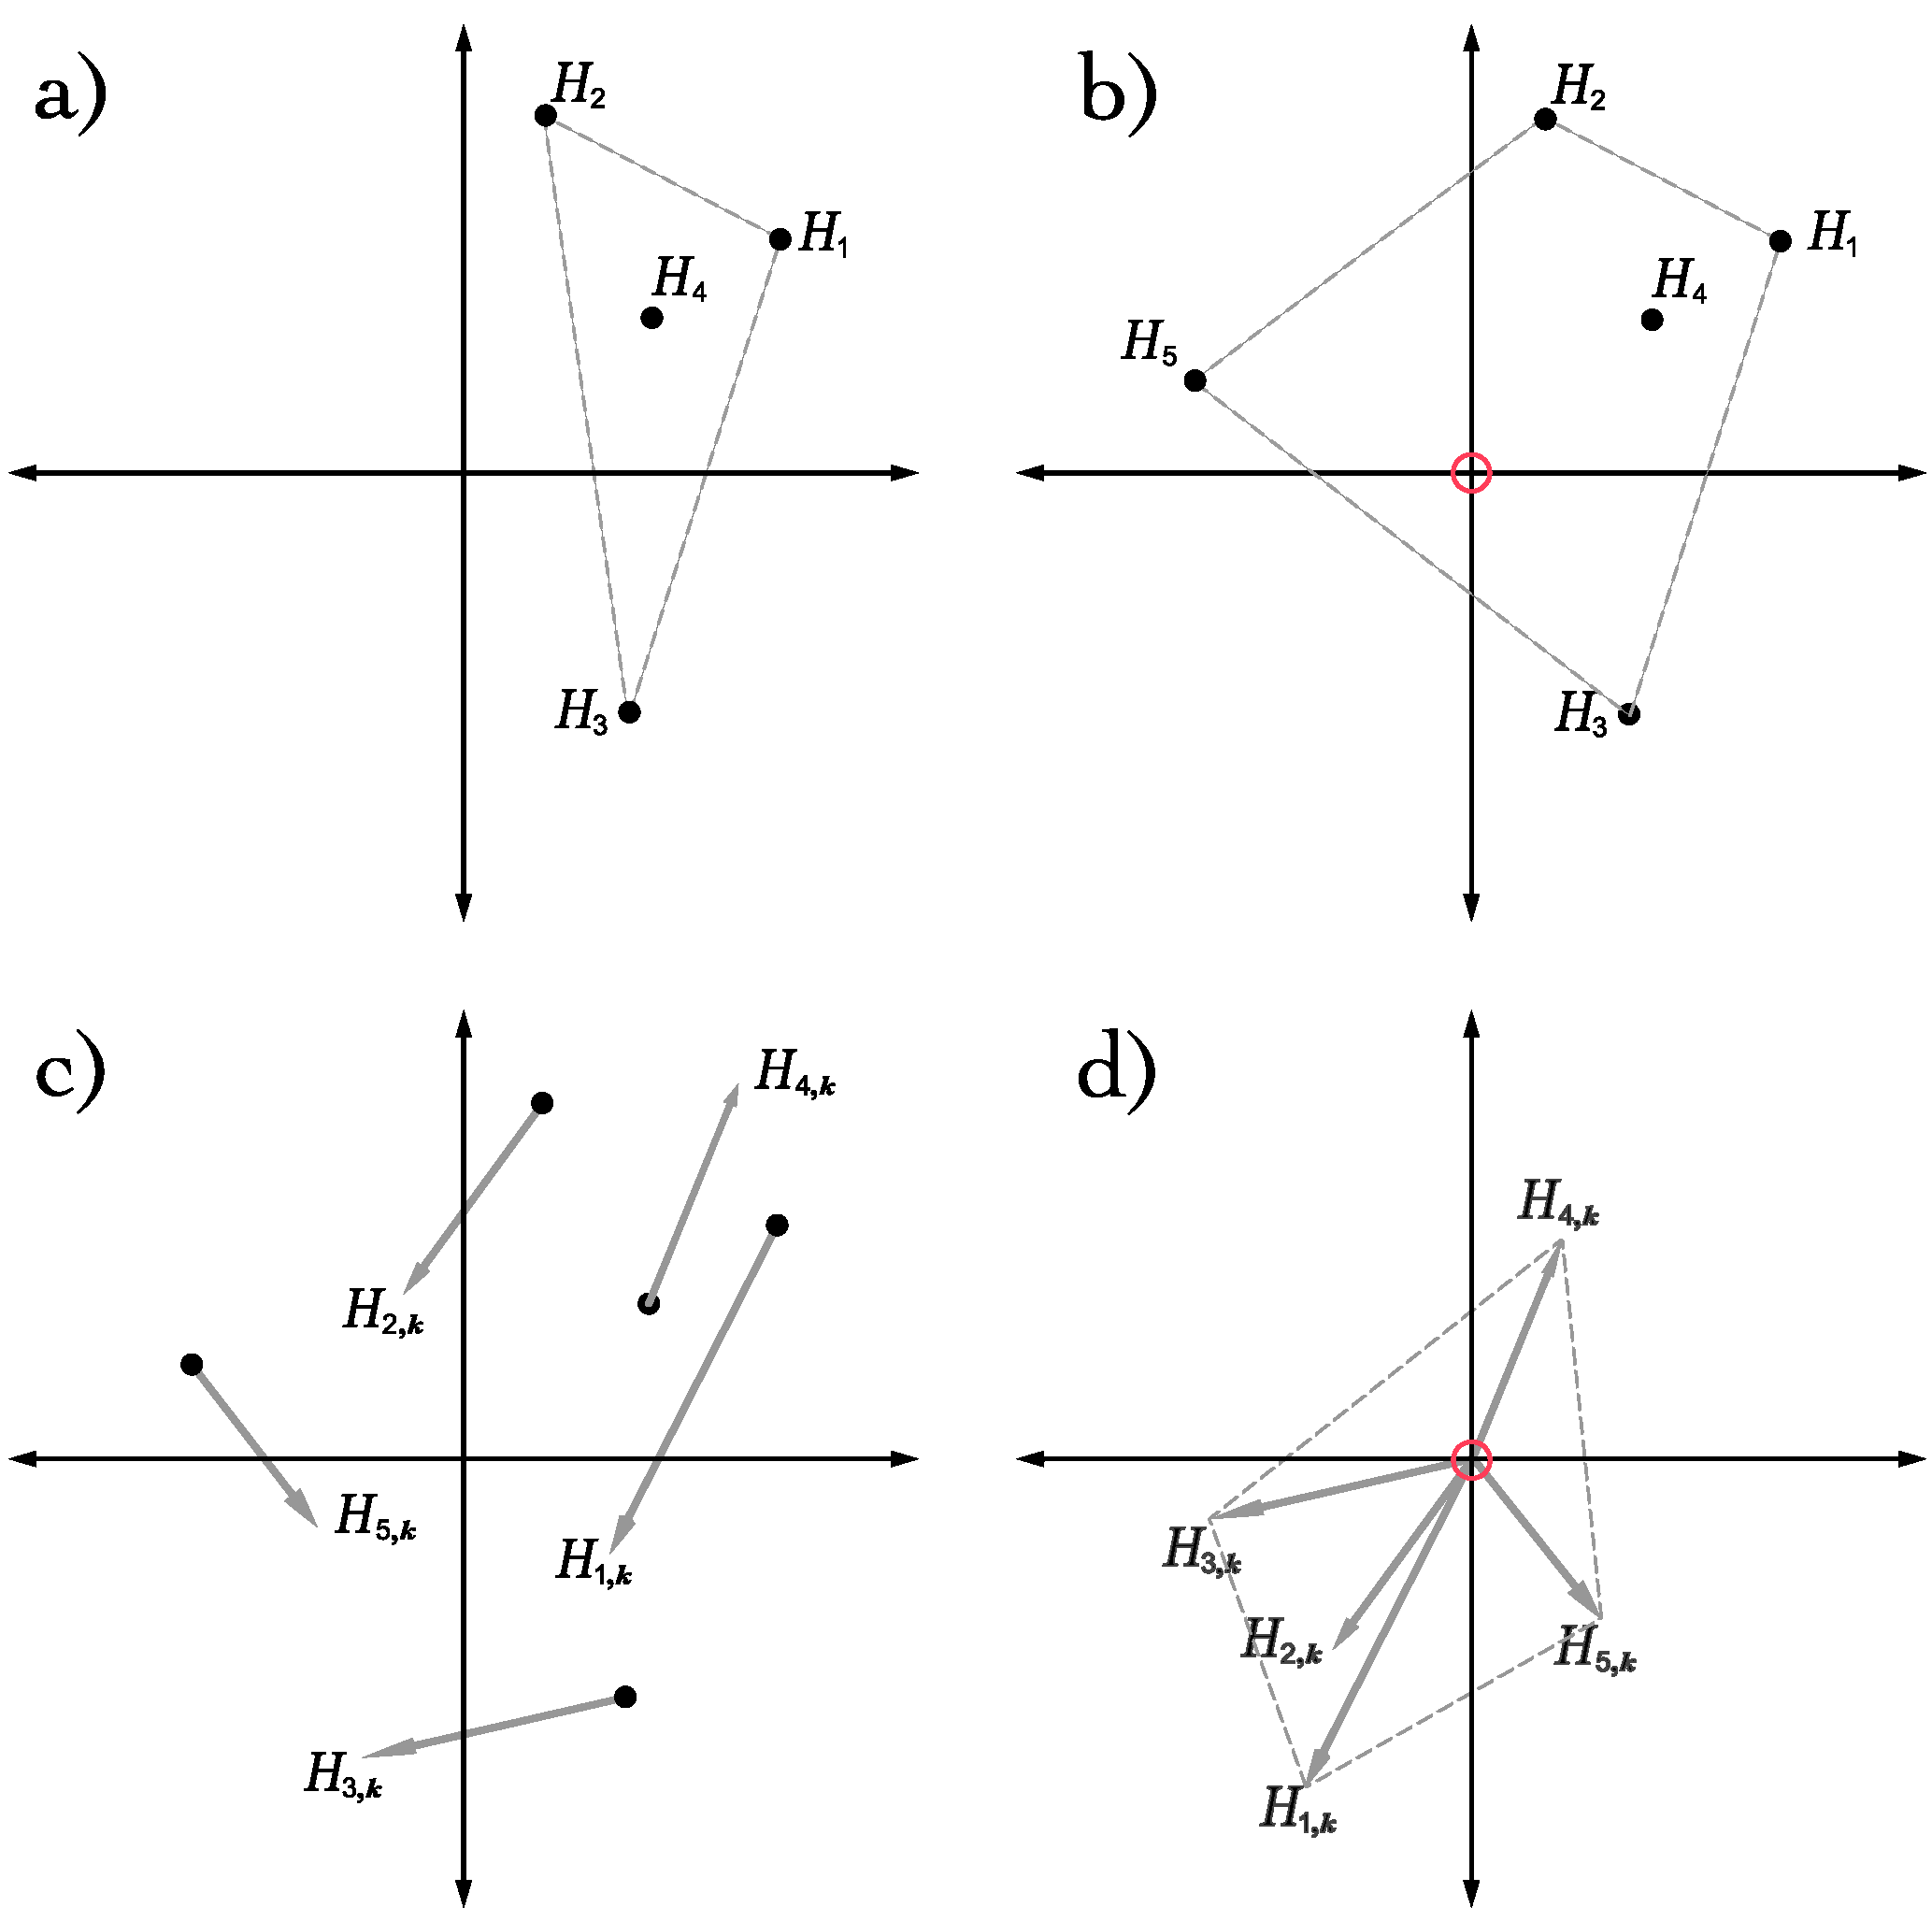
\includegraphics[width=\columnwidth]{vectorspace.pdf}
  \caption{A target unitary gate can be implemented a number of ways, each with a different effective Hamiltonian error. These error Hamiltonians lie in a vector space. a) Four effective Hamiltonians. The origin is not contained in their convex hull, so there are no balanced control solutions. b) The origin is contained in the covex hull after adding an additional control solution. Because there are more than $n+1$ implementations, there exist an infinite number of balanced control solutions. c) The error Hamiltonians shown with their derivative with respect to a control parameter. As this parameter drifts, a $0^{\rm th}$-order balanced control solution may drift, leading to a first-order error. d) The derivatives also lie in a vector space. If the origin lies in their convex hull, then it may be possible to construct a $1^{\rm{st}}$-order mixed unitary process.}
  \label{fig:vectorspace}
\end{figure}

The problem of minimizing $\sin\theta\cos\theta$ can equivalently be cast as trying to construct a family of vectors, $\sin\theta\cos\theta(H_i\sigma_k - \sigma_jH_i)$ whose convex hull contains the origin. This can be seen in Figure \ref{fig:vectorspace} a) and b).

In addition to the type of errors, we care about the size of an error. The \emph{size} of an error in quantum gates may  be quantified in a number of ways. Two of the most common metrics are the average gate fidelity, $\mathcal{F}$, and the diamond norm, $\vert\vert\cdot\vert\vert_\diamond$. These may be represented in terms of the error maps as
\begin{equation}
	\vert\vert I - \error \vert\vert_\diamond = \sup_\rho \vert \vert (I\otimes I)(\rho) - (\error \otimes I)(\rho) \vert\vert_1
\end{equation}
\begin{equation}\label{eq: fid}
	\mathcal{F}(\error) = \frac{\tr{\error} + d}{d^2 + d}
\end{equation}
Which metric is relevant depends on the application, and can yield very different numbers. For instance, the diamond norm is generally linear in the over-rotation angle of a quantum operation, while the average gate infidelity (AGI), given by 1-$\mathcal{F}$, is generally quadratic in the over-rotation angle of a quantum operation. Similarly, these two metric perform very differently on stochastic quantum processes, that can be achieved by probabilistically mixing unitary operators.

A \textit{mixed unitary process} (MUP) consists of a set of unitary channels, $\actual_j$, and associated weights, $\sum_j \omega_j = 1$.  The process matrix for a mixed unitary channel is then the weighted sum of the component channels, $\actual_{\rm M} = \sum_j \omega_j \actual_j$, and the associated error channel is simply the weighted sum of the associated error channels, $\error_{\rm M} = \sum_j \omega_j \error_j$. From this definition, we can compute the AGI of a MUP, by first computing the AGI of an convex combination of channels:
\begin{align}
\mathcal{F}(\alpha\error_1 + (1-\alpha)\error_2) &= \frac{\tr(\alpha\error_1 + (1-\alpha)\error_2) + d}{d^2 + d} \\
&= \alpha\frac{\tr(\error_1) + d}{d^2 + d} + (1-\alpha)\frac{\tr(\error_2) + d}{d^2 + d} 
\end{align}
where we have used the linearity of the trace.
%\begin{align}
%\mathcal{F}(\error_{\rm M}) &= \mathcal{F}(\sum_j \omega_j \error_j)\\
%&= \frac{\tr (\sum_j \omega_j \error_j) + d}{d^2 + d}\\
%&= \frac{\sum_j(\tr (\omega_j \error_j)) + d}{d^2 + d}\\
%&= \frac{\sum_j(\tr (\omega_j (\error_j + d))}{d^2 + d}\\
%&= \sum_j\frac{(\tr (\omega_j (\error_j + d))}{d^2 + d}\\ 
%\end{align}

We therefore see that the AGI of any MUP will be the convex sum of the consituent fidelities, with the same weighting. The diamond norm, however, is non-linear, and can in general be smaller for a MUP than any of the processes being mixed. 

Campbell\cite{Campbell2017} considered this important problem of minimizing the diamond norm of the resulting error channel. Given a collection of component channels with error at most $\epsilon$, they show that if the Hamiltonians form a convex set containing the origin, then the diamond norm can be quadratically supressed. The diamond norm is a particularly appealing target because the it provides useful error metrics on quantum circuits. However, it is not the only optimization target that can be chosen. If the ultimate goal is to produce a channel whose effect can be Monte Carlo simulated, then it may be useful instead to construct a channel whose errors are Pauli stochastic. Using a constrained numerical optimization routine, such a channel could be produced by minimizing the off-diagonal elements of $R$ in Equation \ref{eq:process_matrix}. Indeed, this is the approach we consider in Section \ref{sec:experimental_results}. More generally, the are a number of options one may wish to consider when selecting weights to prepare a mixed unitary process.


% ==============================================================================
% Section: Constructing Useful Unitary Processes
% ==============================================================================
\section{Constructing Useful Unitary Processes}
\label{sec:mixed_unitary_processes}
\subsection{Mixed Unitary Processes with Small Diamond Norm}
\label{sec:small_diamond_norm}
There are often many possibly ways of implementing any given target quantum gate. Campbell and Hastings, for instance, consider gates compiled using the Solovey-Kitaev algorithm, for which many approximate gate compilations are possible.\cite{Campbell2017, 1612.01011} By selecting from these various implementations at random, they show that the resulting quantum channel can be made to have significantly reduced coherent error.  As a simple example of how this occurs, consider a scenario in which we have a single-qubit and four possible implementations of a $\pi$-pulse about the $\sigma_x$ axis. The error channels for these four implementations are themselves unitary rotations about the $\sigma_x$ axis with rotation angles of $\{-2\epsilon, -\epsilon, \epsilon, 2\epsilon\}$. Such a situation could appear, for instance, if there were amplitude errors on the fields used to affect the gates, and if the control could be implemented by a rotation about the positive or negative $\sigma_x$ axis.

\begin{center}

\begin{tabular}{cccc}
	Gate & $H_{\rm{eff}}$ & AGI & $\vert\vert\cdot\vert\vert_\diamond$ \\
\hline
	$U_{+2\epsilon}$ & $2\epsilon \sigma_x$ & $4\epsilon^2$ & $2\epsilon$\\
	$U_{+\epsilon}$ & $\epsilon \sigma_x$ & $\epsilon^2$ & $\epsilon$ \\
	$U_{-\epsilon}$ & $-\epsilon \sigma_x$ & $\epsilon^2$ & $\epsilon$ \\
	$U_{-2\epsilon}$ & $-2\epsilon \sigma_x$ & $4\epsilon^2$ & $2\epsilon$ 
\end{tabular}

\end{center}

\begin{figure}
  \centering
  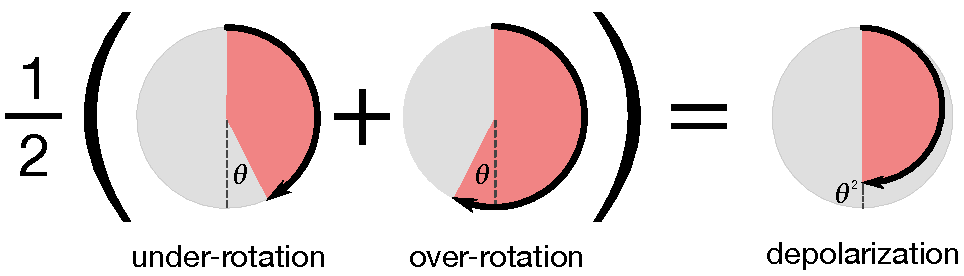
\includegraphics[width=\columnwidth]{simple_example.pdf}
  \caption{An example of a mixed unitary process. Using optimal control, two implementations of a $Z_\pi$ gate are designed to have equal and opposite sensitivity to errors (if one implementation over-rotates by angle $\theta$, then the other \emph{under}-rotates by $\theta$). Each time the gate is used, one of these implementations is chosen at random. The resulting quantum channel is equivalent to a perfect implementation of the gate followed by dephasing of $\order{\theta^2}$.}
  \label{fig:simple_example}
\end{figure}

In this case, the MUP that minimizes the diamond norm is given by:
\begin{equation}
\frac{1}{2}U_{+\epsilon}^*\otimes U_{+\epsilon} + \frac{1}{2}U_{-\epsilon}^*\otimes U_{-\epsilon}
\end{equation}
More generally, the problem remains: given a collection of channels, how can one efficiently compute a weighting that minimizes a particular metric?

As discussed in \cite{Campbell2017}, a sufficient condition to minimize the diamond norm of a MUP with error generators $\{H_j\}$ to first order is:
\begin{equation}\label{eq:campbell-condition}
\sum \omega_j H_j = 0
\end{equation}
In \cite{Campbell2017} Campbell constructs an algorithm that, given an oracle to approximate unitaries, finds a MUP with this property. Alternatively, one can use convex optimization to solve this problem. Consider the matrix whose rows are the vectorized Hamiltonians at our disposal, i.e. for $m$, $n\times n$ Hamiltonians:
\begin{equation}\label{eq:vectorized_hamiltonians}
	H = \left(\begin{array}{cccc}
		H_{1_{11}} & H_{2_{21}} & \ldots   \\ 
		\vdots\ & \ddots &    \\
		H_{m_{11}} &  &  H_{m_{nn}} \\ 
	\end{array} 	
	\right)
\end{equation}
If our weighting vector for our MUP is $\omega$, we can rewrite this sum as a matrix product whose two-norm will be zero if and only if the sum is zero. That is, we can instead consider solving the following convex optimization problem:

\begin{equation}\label{eq:minimization}
  \begin{split}
    &\underset{\omega_j\geq0, |\omega|_1=1}{\textbf{minimize}: } ||H^T\omega||_2\\
  \end{split}
\end{equation}
where the minimization is over all valid probability distributions.
\subsection{Robustly Mixed Unitary Processes}
\label{sec:robustly_mixed}

While mixed unitary processes offer significant improvements to gate performance, they fail to take into account the reality that most control electronics experience drift over time scales relevant to QIP performance. Because of this drift, the quality of the MUP will degrade. Thus, we would like to design MUPs that are \textit{robust} to this drift. To enforce robustness, we can consider higher derivatives of the Hamiltonians in \ref{eq:campbell-condition}. Instead of just requiring that the $0^{th}$ derivative averages to zero, we should impose a similar condition on the derivatives of the Hamiltonians with respect to parameters that may drift:
\begin{equation}
D^n_j = \frac{1}{n!}\frac{\partial^{n}}{\partial\delta_{i_1}\ldots\partial\delta_{i_n}}H_j(\vec{\delta})|_{\delta=\vec{0}}
\end{equation}
Then we say that a mixed unitary process is said to be robust to order $\ell$ (an $\ell$MUP) if for all $1 \leq j \leq \ell$:
\begin{equation}\label{eq:MUP}
\begin{gathered}
\sum_j\omega_j(\sum_{n=0}^k D^n_j)^k = 0\\
\end{gathered}
\end{equation}
In particular, we see that a 0MUP satisfies Equation \ref{eq:campbell-condition}. More generally, these conditions imply that an $\ell$MUP is insensitive to the $\ell^{th}$ order in drift in $\vec{\delta}$. To see this, we can rewrite the error on each control in the MUP as:
\begin{equation}\label{eq:taylor}
\begin{gathered}
\actual_j(\vec{\delta}) = \exp(-i(H_j(\vec{0}) + \frac{\partial}{\partial\delta_i}H_j(d\delta_i)\\ +  \frac{1}{2}\frac{\partial^2}{\partial\delta_i\partial\delta_k} H_j(d\delta_i d\delta_k) + \ldots))\target
\end{gathered}
\end{equation}
By Taylor expanding Equation \ref{eq:taylor} in $\vec{\delta}$, one finds that the the first $\ell$ derivatives of an $\ell MUP$ will be zero. Furthermore, if we are only interested in being first order insensitve to drift and can select controls such that $|D_j^n|\approx\epsilon$, we see that Equation \ref{eq:MUP} can be approximated as:
\begin{equation}\label{eq:MUP-relaxed}
\begin{gathered}
\sum_k\omega_jD^n_j = 0\\
\end{gathered}
\end{equation}
This condition guarantees that errors will be supressed quadratically for all derivatives up to order $\ell$. Following from Lemma 2 in \cite{Campbell2017}, if $0\in $ Conv$[\{H_i(\vec{\delta})\}]$, where Conv is the convex hull of its arguments, then we know that an $\vec{\omega}$ exists that quadratically decreases the diamond norm. This condition is illustrated in Figure \ref{fig:vectorspace} gives geometric intuition for the conditions required to produce an $\ell MUP$.

To generate robustly mixed unitary processes, we first define the vectorized derivative matrix ${D^{\ell}}$ in a similar way to \ref{eq:vectorized_hamiltonians}:
\begin{equation}
{D^{\ell}}^T =  \left(\begin{array}{cccc}
		D^\ell_{1_{11}} & D^\ell_{2_{21}} & \ldots   \\ 
		\vdots\ & \ddots &    \\
		D^\ell_{m_{11}} &  &  D^\ell_{m_{nn}} \\ 
	\end{array} 	
	\right)
\end{equation}

Using this, we can then solve the following convex optimization problem, generalizing Equation \ref{eq:minimization}:

\begin{equation}\label{eq:robust_minimization}
  \begin{split}
    &\underset{\omega_j\geq0, |\omega|_1=1}{\textbf{minimize}: } ||{D^{\ell}}^T\omega||\\
    &\textbf{subject to: } \forall n<\ell, \sum \omega_jD_j^n=0\\
  \end{split}
\end{equation}
with $D_k^n$ defined in Equation \ref{eq:MUP}. 

\subsection{Hamiltonian Norm Regularization}
While these particular convex optimization problem can be solved through a system of linear equations, casting it as a convex optimization problem allows us to regularize the cost function, and introduce additional constraints. In particular, while this minimization problem is sufficient for quadratically decreasing the diamond norm relative to the \textit{worst} controls in the collection, it does not preferentially select the controls with the least error. That is to say, both \{$U_{+2\epsilon}$, $U_{-2\epsilon}$\} and \{$U_{\epsilon}$, $U_{-\epsilon}$\} from Section \ref{sec:small_diamond_norm} satisfy Equation \ref{eq:minimization}. To encourage the inclusion of controls with smaller error, we may impose an $\ell_2$ penalty to our cost function by rewriting it as:

\newcommand{\bunderbrace}[2]{%
  \begin{array}[t]{@{}c@{}}
  #1\\
  \parbox{\widthof{#1}}{$\scriptscriptstyle#2$}
  \end{array}
}

\begin{equation}\label{eq:minimization_l2}
\begin{split}
&\underset{n\in[N]}{\textbf{minimize}}\{\\
&\ \ \bunderbrace{\textbf{minimize}: }{\omega_j\geq0, |\omega|_1=1} ||{D^{\ell}}^T\omega||+ \eta\sum\omega_j||D^0_j||_2\\
&\ \ \textbf{subject to: } \forall n<\ell, \sum \omega_jD_j^n=0\\
&\}
\end{split}
\end{equation}
with $\eta \geq 0$. By making $\eta$ larger, we can require that the solver decreases the diamond norm of the constituent channel, while using only the best controls.



%\begin{equation}\label{eq:minimization_l2}
%  \begin{split}
%    &\underset{\omega_j\geq0, |\omega|_1=1}{\textbf{minimize}: } ||D_{\ell}^T\omega||_2 + \eta\sum||D_0^T\omega||_2\\
%  \end{split}
%\end{equation}
\subsection{Sparsity Constraints}
As a practical consideration, we would also like to regularize our objective function to enforce sparsity. Control electronics often have a limited amount of waveform memory, and thus it is important that MUPs have non-trivial probability support on a small number of controls. As an example of where this would be necessary is Figure\ref{fig:vectorspace}. In Subfigure b, it's clear that $H_4$ is unecessary to contain the origin in the convex hull of the error generators. However, if we additionally want our controls to form a 1MUP, we see from Subfigure D that we need $H_4$ in our control set. Thus we would like the solver to be frugal in which controls it selects. In many machine learning situation, lasso regularization \cite{tibshirani1996regression} can be used to enforce sparsity, however here it is insufficient as we already constrain the one norm of the vector we optimize over to be one. Conveniently, the problem of enforcing sparsity in such situations has been considered in \cite{NIPS2012_4504} and can be expressed via another convex program that extends Equation \ref{eq:minimization}:

\begin{equation}\label{eq:minimization_regularization}
\begin{split}
&\underset{n\in[N]}{\textbf{minimize}}\{\\
&\ \ \bunderbrace{\textbf{minimize}: }{\omega_j\geq0, |\omega|_1=1,\\ t\geq0} ||{D^{\ell}}^T\omega|| + t\\
&\ \ \textbf{subject to: } \omega_n > \frac{\lambda}{t}\\
&\ \ \phantom{\textbf{subject to: }} \forall n<\ell, \sum \omega_jD_j^n=0\\
&\}
\end{split}
\end{equation} where $\lambda$ is a hyperparameter to be optimized over.


% ==============================================================================
% Section: Numerical Results
% ==============================================================================
\section{Numerical Results}
\label{sec:numerical_results}
\label{one_qubit_performance}
In the following numerical results, we explore using the methods in Section \ref{sec:mixed_unitary_processes} to build MUPs. We consider the following model for a single tunable qubit: 
\begin{equation}\label{eq:1Qham}
  H(\delta, \epsilon, t) = \epsilon\sigma_z + (1 + \delta)(c_x(t)\sigma_x + c_y(t)\sigma_y)
\end{equation}
We use the GRAPE algorithm as discussed in Section \ref{sec:random_gate_synthesis} with N=25 steps and total evolution time of $\pi$ to generate 100 candidate controls, with a standard deviation of $\sigma=.001$ for the distribution in Equation \ref{eq:quadrature}. We assume that the errors on $\sigma_x$ and $\sigma_y$ are perfecly correlated, as is the case in systems that implement RZ rotations with phase shifts of the control signal. Solving the optimization problem defined in Section \ref{sec:robustly_mixed} yields similar MUPs for $RX(\frac{\pi}{2})$ and $RY(\frac{\pi}{2})$, with the results for $RY(\frac{\pi}{2})$ shown in Figure \ref{fig:YMUP}. These results demonstrate several properties that make MUPs both useful and tractable.


First, naively generating a 0MUP results in nontrivial support on all the members of the control family. However, by rewriting the minimization to impose the sparsity constraint discussed in Section \ref{sec:robustly_mixed}, we can generate a 0MUP that uses just five of the controls. This shows that through adding constraints to our optimization routine, we can make the MUP practically useful. In both cases we impose the same $\ell_2$ penalty as described in Section \ref{sec:robustly_mixed}, so that the algorithm preferentially selects controls with smaller errors. Imposing this constraint allows us to trade off flatness at the origin for performance.
\subsection{Two Qubit Performance Analysis}
\label{two_qubit_performance}
In our two-qubit example we consider the following model for two tunable qubits coupled by a resonant exchange interaction, similar to that in \cite{McKay2016}:
\begin{equation} \label{eq:2Qham}
\begin{split}
H(\vec{\delta}, \vec{\epsilon}, t) = &\sum_{j=1}^2(\epsilon_j\sigma_z^j + (1 + \delta_j)(c_x^jx(t)\sigma_x^j + c_y^j(t)\sigma_y^j)) \\
&+ \frac{1}{10}(XX + YY)
\end{split}
\end{equation}

In this example it was infeasible to use GRAPE to return non-trivial solutions. Instead we manually selected piecewise constant echoing sequences with 500 steps and total evolution time of $\frac{5\pi}{2}$. In particular, we considered $RX(\pi)$, $RX(-\pi)$, $RY(\pi)$ and $RY(-\pi)$ bang-bang sequences \cite{bangbang}, consisting of all combinations of simultaneous $\pi$ pulses activated at multiples of $8$ steps from the beginning of the controls, and the same multiple of $8$ steps prior to the end of the controls. An example of such a control is given in Figure \ref{fig:bangbang}. To give the control family a variety of RF errors, we added on uniformly distributed errors to each $\pi$ pulse, between $-.25$\% and $.25$\%.


\begin{figure}
  \centering
  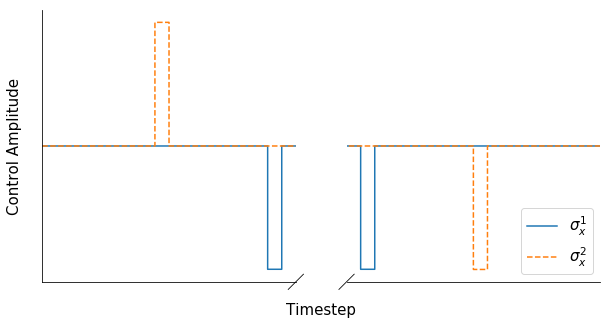
\includegraphics[width=\columnwidth]{bangbang.png}
  \caption{Example bang-bang sequence, using both qubits' $\sigma_x$ controls. Not shown are the unused $\sigma_y$ controls, and the uncontrolled resonant exchange interaction.}
  \label{fig:bangbang}
\end{figure}


In this example, we find more modest improvements to performance, as shown in Figure \ref{fig:2MUP}. There are now four free parameters to optimize over, and the uncontrolled entangling interaction means that there is little room for variation in the controls. Nonetheless, using a MUP improves performance by half of an order of magnitude at the origin relative to the constituent controls, and up to an order of magnitude away from the origin. For all values of the drifting parameters we see that the 1MUP performs as well or better than 0MUP.

% ==============================================================================
% Section: Experimental Results
% ==============================================================================

\section{Experimental Results}
\label{sec:experimental_results}
Here we present experimental results from implementing our routine on a fixed-frequency superconducting transmon qubit. In particular, we used qubit 8 on the Rigetti 19Q-Acorn chip, whose characterization can be found in \cite{1712.05771}. To implement a MUP on this qubit, four incorrectly calibrated Gaussian pulses were produced by scaling the pulseshape amplitude for a calibrated 10 sample 50ns $RX(\frac{\pi}{2})$ pulse by $106.4\%$,  $103.9\%$, $93.7\%$ and $91.2\%$.


\begin{figure}
  \centering
  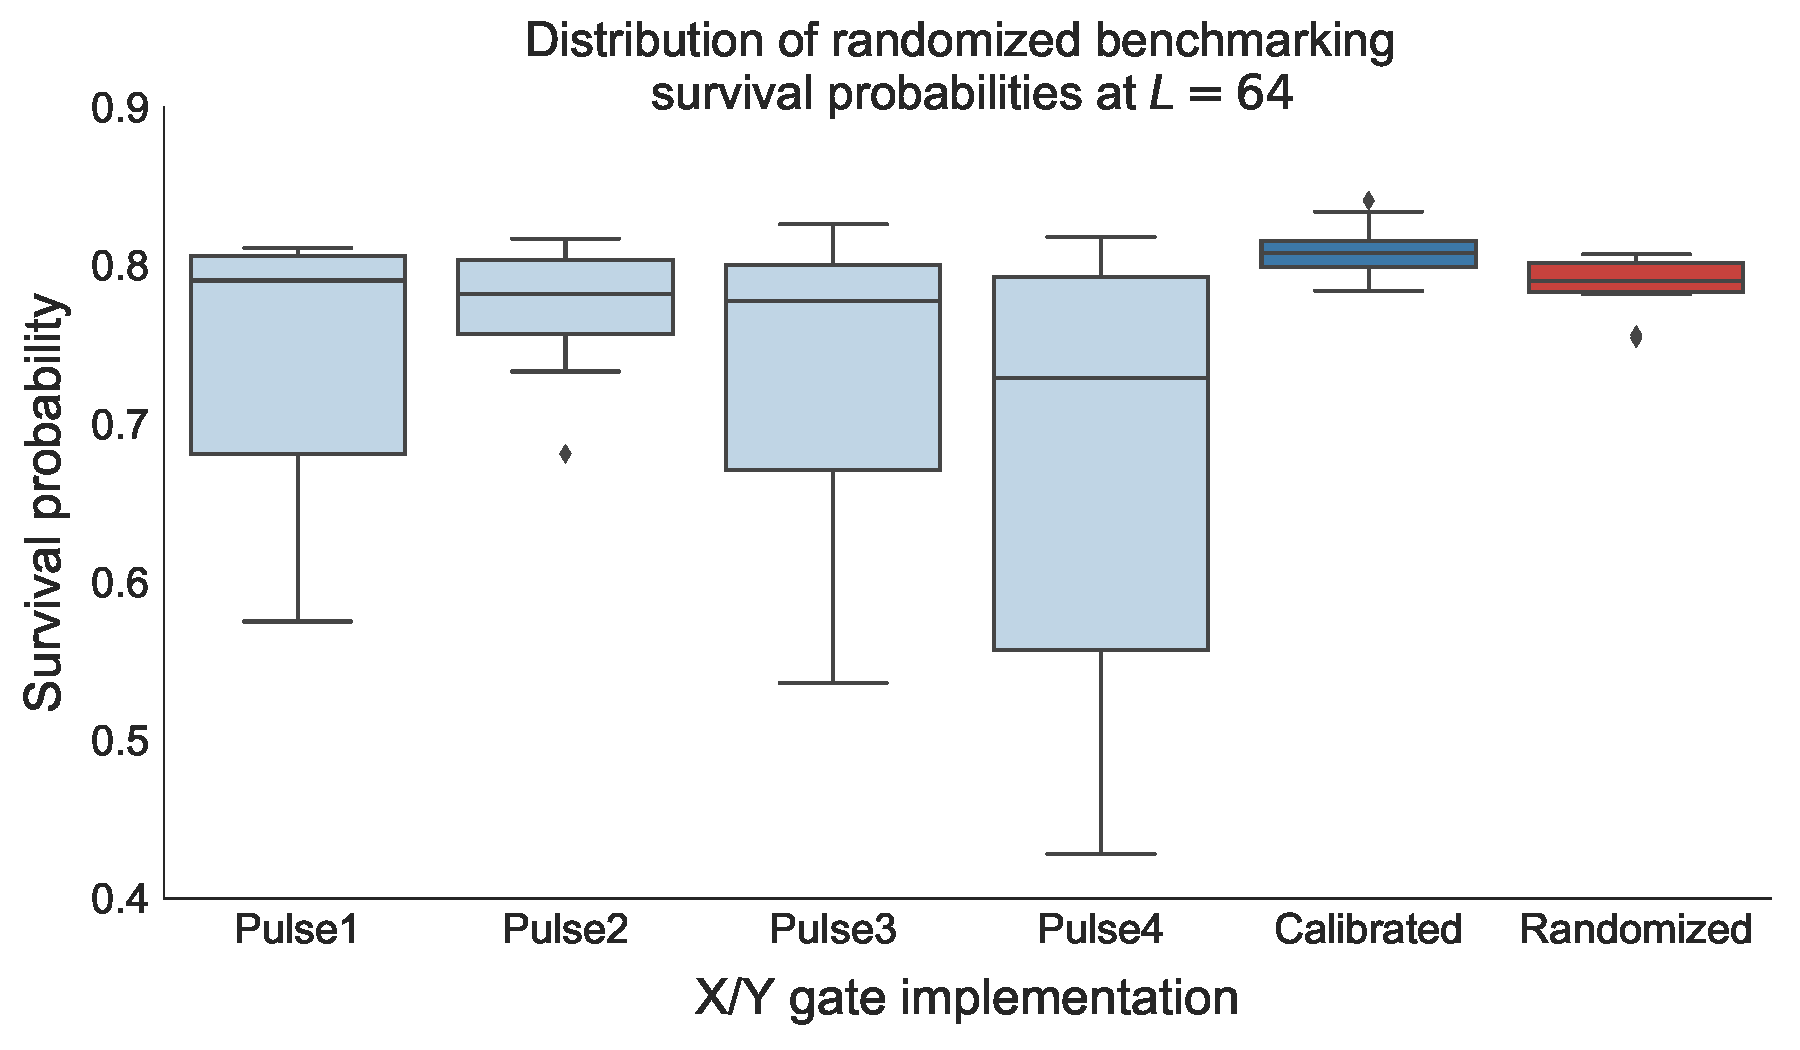
\includegraphics[width=\columnwidth]{rb_data.pdf}
  \caption{Randomized benchmarking experiments ran using different pulse definitions. The four plots on the left are from the incorrectly calibrated pulse, while the top right is the calibrated pulse, and the bottom right is the MUP.}
  \label{fig:rb}
\end{figure}


As discussed in Section \ref{sec:robustly_mixed}, we chose here to minimize the off diagonal elements of the process matrix. To benchmark the quality of the MUP, we then performed six randomized benchmarking experiments\cite{Magesan2011}: one for each over-- and under--calibrated pulse, one for the calibrated pulse, and one for the mixed process. We used $1000$ shots per experiment, $10$ sequences per sequence length, for sequence lengths of $2, 4, 8, 16, 32$ and $64$. In each case, our Clifford operations were decomposed into RX($\frac{\pi}{2})$) and RY($\frac{\pi}{2})$) pulses. In our implementation, these gates are implemented using the same pulse envelope definitions and control electronics, phase shifted by $\frac{\pi}{2}$ radians, and are therefore subject to identical miscalibration errors. The results are shown in Figure \ref{fig:rb} for sequence lengths $L=64$. Fitting to the randomized benchmarking decay curves, we find one-qubit gate fidelities of $99.3\%$ for the calibrated pulse, $98.9\%$ for Pulse1, $99.1\%$ for Pulse2, $98.9\%$ for Pulse3, $98.5\%$ for Pulse4, and $99.2\%$ for the MUP, demonstrating that it performs almost as well as the calibrated pulse, and better than the constituent pulses. 

Additionally, by minimizing the off-diagonal elements of the process matrix, rather than balancing the Hamiltonian errors, we expect to produce a process with minimal coherent error in the absence of drift. To see that this is the case, we cite the results in \cite{Ball2016}. For non-Markovian error models, noise will manifest as gamma distributed points for each sequence length. On the other hand, Markovian noise, such as depolarizing noise, will result in Gaussian distributed fidelity estimates for each randomized benchmarking sequence length. We see that the coherently miscalibrated controls in our RB experiment have long tails, consistent with gamma distributed random variables, while the calibrated and randomized implementations both have much shorter tails, consistent with Gaussian distributed random variables. Thus, our experiment demonstrates that not only is the performance of the MUP better than the constituent gates, it also has a signicantly less-coherent error channel.


% ==============================================================================
% Section: Conclusion and Future Work
% ==============================================================================


\section{Conclusion and Future Work}
We have shown numerically that using MUPs can reduce coherent error on a quantum channel by more than an order of magnitude in diamond norm, over a wide range of quasi-static values of noise. In addition, we have demonstrated that these approximate controls can be generated through optimal control (GRAPE), and that the minimization problem is tractable.

Future directions for this work include demonstrating the routine experimentally on a two-qubit gate, moving the random gate selection from a precompilation step to runtime logic onboard the control electronics, investigating other optimization routines such as CRAB \cite{Caneva2011} and GOAT\cite{Machnes2018}, and using more sophisticated benchmarking routines such as GST\cite{BlumeKohout2017} to quantitatively investigate the performance of our method.

Another interesting area of research would be using model-free approaches. The numerical work in the paper assumes access to a model of the system, however an experimentalist may not have a model readily available to describe the system, e.g. in the presence of unknown on-chip crosstalk, or an uncalibrated transfer function of the system. Even if a model is available, it might be computationally inconvenient to simulate, i.e. for more than a few qubits.

In these situations, one approach would be to use \textit{in-situ} optimal control techniques \cite{Wu2018, Kelly2014, Ferrie2015} to generate candidate controls, and then use an optimizer like Nealder-Mead to perform the minimization. While performing a complete optimization in this way would require full process tomography, one could intead optimize via partial tomography. By selecting pre-- and post --rotations that correspond to measuring Pauli-moments of interest in the Hamiltonian, such as unwanted $Z\otimes Z$ crosstalk, one could perform optimization over fewer parameters.


% ==============================================================================
% Section: Acknowledgements
% ==============================================================================
\section{Acknowledgements}
\label{sec:acknowledgements}
Sandia National Laboratories is a multimission laboratory managed and operated by National Technology and Engineering Solutions of Sandia, LLC, a wholly owned subsidiary of Honeywell International, Inc., for the U.S. Department of Energy's National Nuclear Security Administration under contract DE-NA0003525.
\bibliography{decorrelation.bib}


\newpage
\onecolumngrid
% ==============================================================================
% Section: Appendix
% ==============================================================================
\section{Appendix}
\label{sec:appendix}
\begin{figure*}[h]
  \centering
  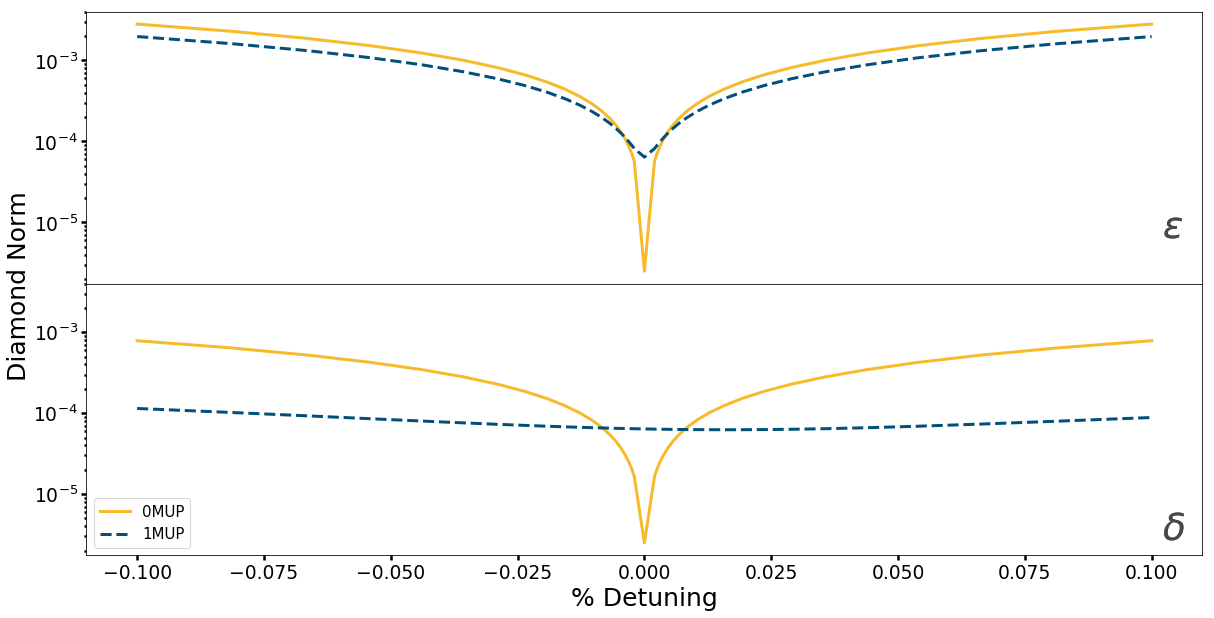
\includegraphics[width=\textwidth]{SQRTY_no_member.png}
  \caption{Numerical results comparing a 0MUP to a 1MUP for a single tunable qubit, for $RY(\frac{\pi}{2})$. The results are qualitatively similar to those for $RX(\frac{\pi}{2})$. In this case the 0MUP outperforms both the 1MUP by two orders of magnitude, and the constituent controls by three orders of magnitude at the origin. However, varying over $\delta$ we see that the 1MUP outperforms the 0MUP by up to an order of magnitude when there is $.1\%$ drift in the qubit control amplitudes.}
  \label{fig:YMUP}
\end{figure*}

\begin{figure*}[h]
  \centering
  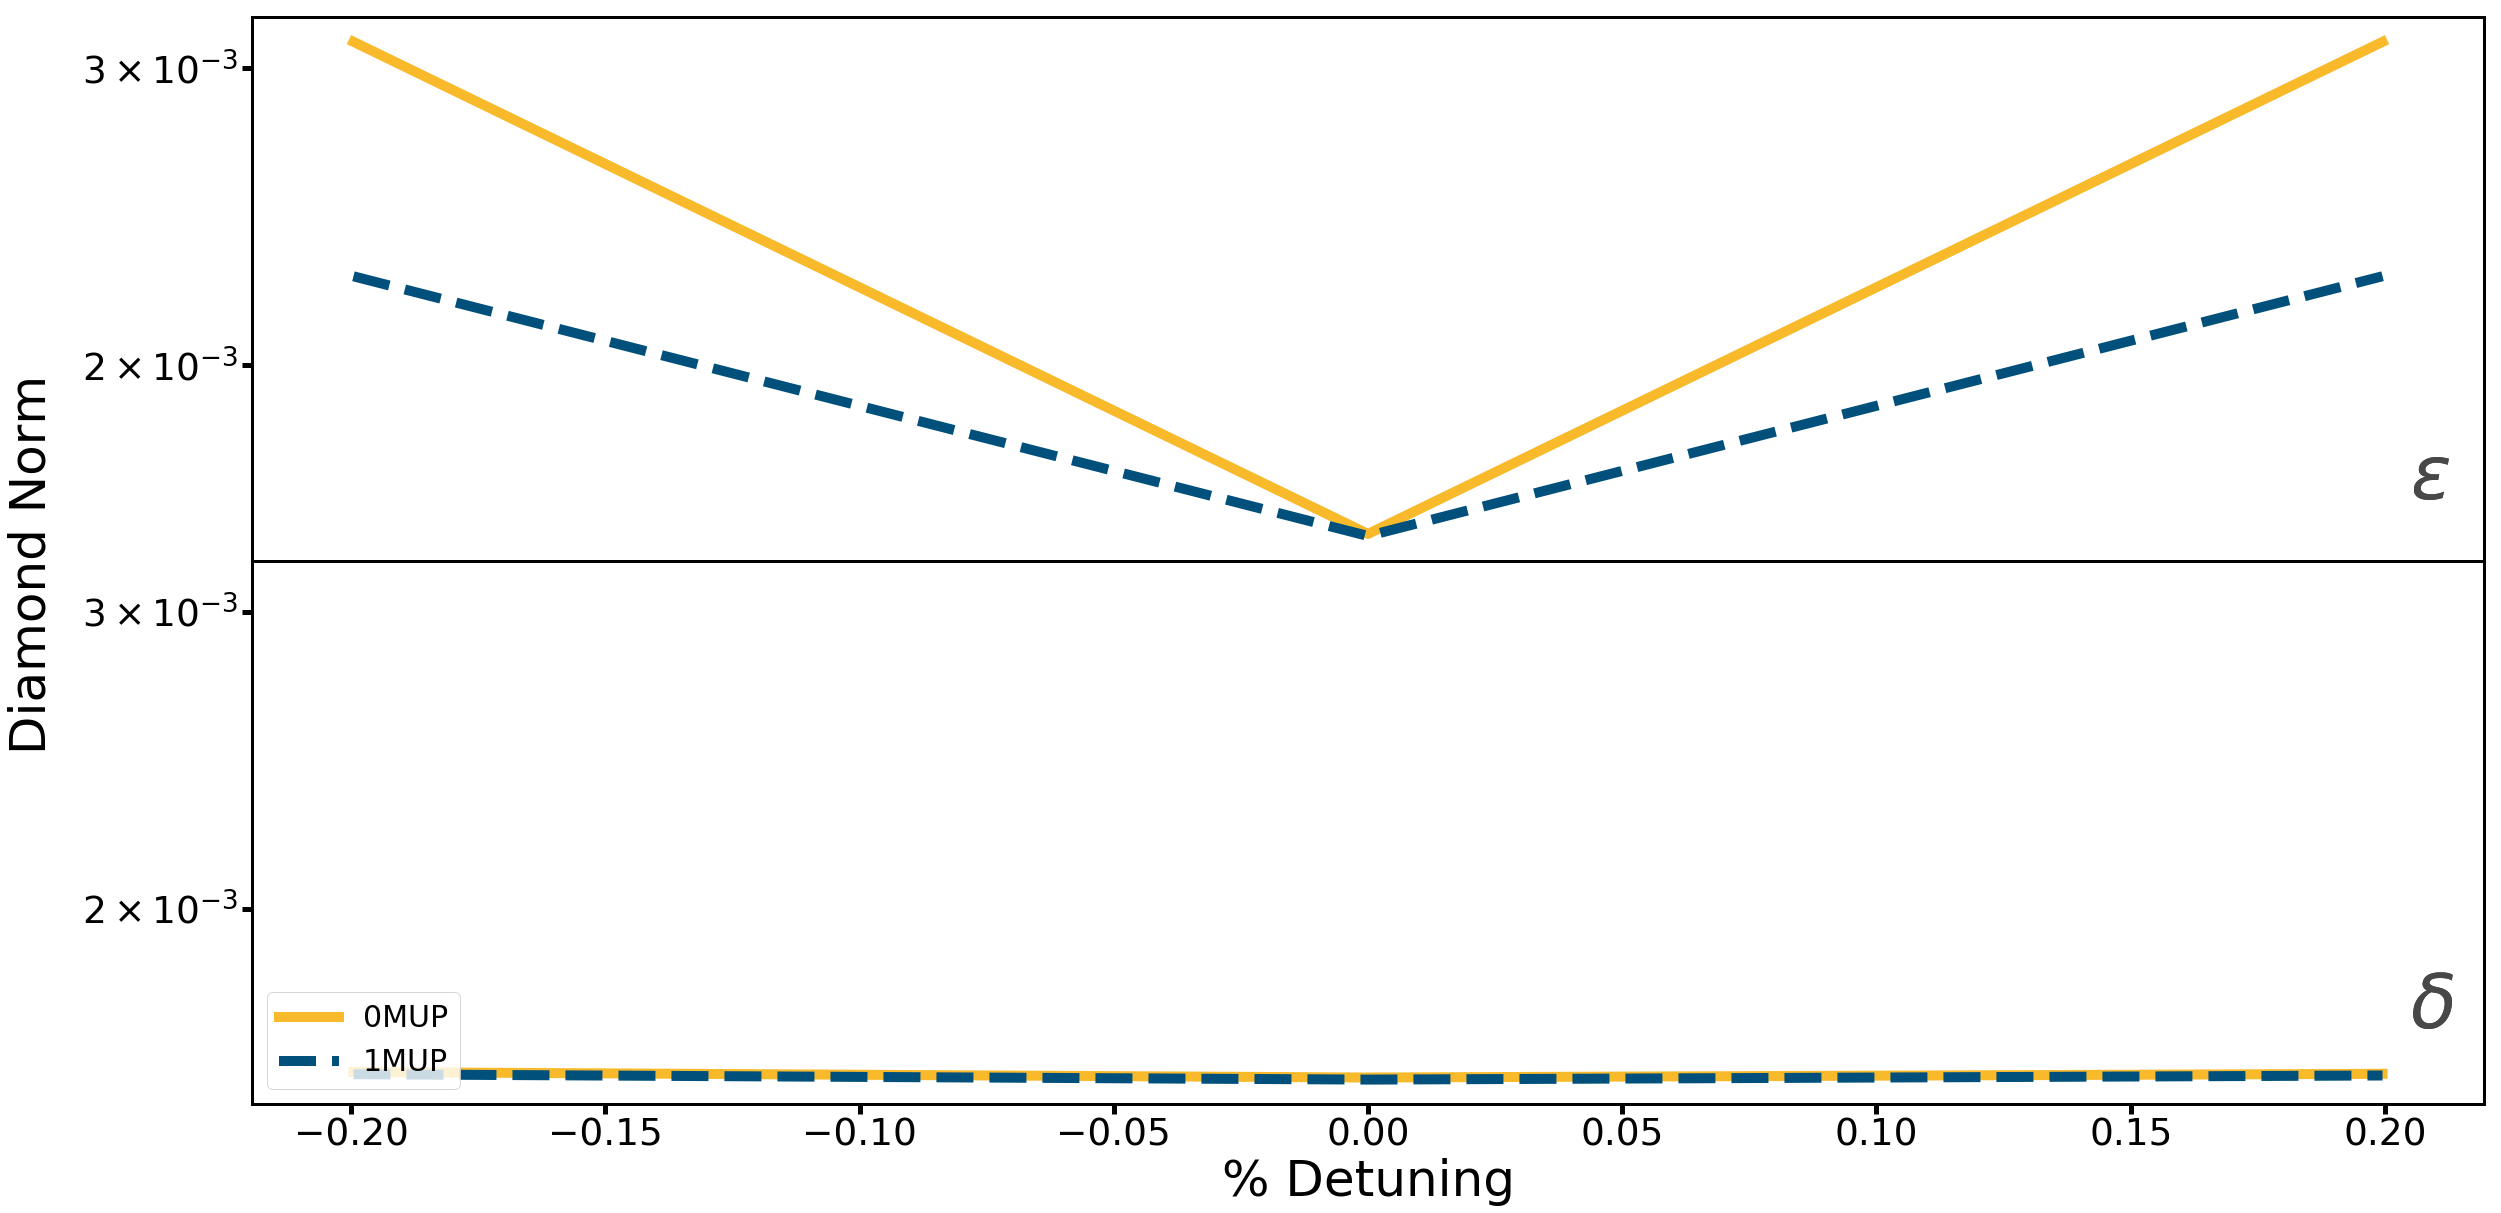
\includegraphics[width=\textwidth]{2QRBC_no_member.png}
  \caption{Numerical results comparing a 0MUP to a 1MUP for a pair of tunable qubits, with a resonant exchange interaction. Shown with lower alpha values are example constituent controls. The 0MUP and 1MUP can be seen to outperform these controls by half of an order of magnitude at the origin. For all detuning values the 1MUP performs as well or better than the 0MUP. When there is $.2\%$ drift in the qubit frequency, the 1MUP outperforms members of the control famlies by almost an order of magnitude in diamond norm. Similarly, for $.2\%$ drift in the qubit control amplitude, we see that the 1MUP outperforms the the constituent controls by over half an order of magnitude.}
  \label{fig:2MUP}
\end{figure*}


\end{document}
